\documentclass[10pt,a4paper,final]{article} %draft

\usepackage[english, russian]{babel}

\usepackage[final]{pdfpages}

\usepackage{textcomp,enumitem}

\usepackage{amsmath,amsthm,amssymb}

\usepackage{listings}
\usepackage{xcolor}
\usepackage{caption}

\definecolor{codegray}{rgb}{0.95,0.95,0.95}
\definecolor{codepurple}{rgb}{0.58,0,0.82}

\lstset{
	extendedchars=true,
	literate=
	{а}{{\selectfont\char224}}1
	{б}{{\selectfont\char225}}1
	{в}{{\selectfont\char226}}1
	{г}{{\selectfont\char227}}1
	{д}{{\selectfont\char228}}1
	{е}{{\selectfont\char229}}1
	{ж}{{\selectfont\char230}}1
	{з}{{\selectfont\char231}}1
	{и}{{\selectfont\char232}}1
	{й}{{\selectfont\char233}}1
	{к}{{\selectfont\char234}}1
	{л}{{\selectfont\char235}}1
	{м}{{\selectfont\char236}}1
	{н}{{\selectfont\char237}}1
	{о}{{\selectfont\char238}}1
	{п}{{\selectfont\char239}}1
	{р}{{\selectfont\char240}}1
	{с}{{\selectfont\char241}}1
	{т}{{\selectfont\char242}}1
	{у}{{\selectfont\char243}}1
	{ф}{{\selectfont\char244}}1
	{х}{{\selectfont\char245}}1
	{ц}{{\selectfont\char246}}1
	{ч}{{\selectfont\char247}}1
	{ш}{{\selectfont\char248}}1
	{щ}{{\selectfont\char249}}1
	{ъ}{{\selectfont\char250}}1
	{ы}{{\selectfont\char251}}1
	{ь}{{\selectfont\char252}}1
	{э}{{\selectfont\char253}}1
	{ю}{{\selectfont\char254}}1
	{я}{{\selectfont\char255}}1
	{А}{{\selectfont\char192}}1
	{Б}{{\selectfont\char193}}1
	{В}{{\selectfont\char194}}1
	{Г}{{\selectfont\char195}}1
	{Д}{{\selectfont\char196}}1
	{Е}{{\selectfont\char197}}1
	{Ж}{{\selectfont\char198}}1
	{З}{{\selectfont\char199}}1
	{И}{{\selectfont\char200}}1
	{Й}{{\selectfont\char201}}1
	{К}{{\selectfont\char202}}1
	{Л}{{\selectfont\char203}}1
	{М}{{\selectfont\char204}}1
	{Н}{{\selectfont\char205}}1
	{О}{{\selectfont\char206}}1
	{П}{{\selectfont\char207}}1
	{Р}{{\selectfont\char208}}1
	{С}{{\selectfont\char209}}1
	{Т}{{\selectfont\char210}}1
	{У}{{\selectfont\char211}}1
	{Ф}{{\selectfont\char212}}1
	{Х}{{\selectfont\char213}}1
	{Ц}{{\selectfont\char214}}1
	{Ч}{{\selectfont\char215}}1
	{Ш}{{\selectfont\char216}}1
	{Щ}{{\selectfont\char217}}1
	{Ъ}{{\selectfont\char218}}1
	{Ы}{{\selectfont\char219}}1
	{Ь}{{\selectfont\char220}}1
	{Э}{{\selectfont\char221}}1
	{Ю}{{\selectfont\char222}}1
	{Я}{{\selectfont\char223}}1,
%	{|}{{\textbar}}1,
%	{||}{{\textbar\textbar}}1
%	{\&}{{\string&}}1
%	{==}{{\string==}}1
%	{\string\\}{{\string\\}}1,
	numbers=left,
	stepnumber=1,
	firstnumber=1,
	numberstyle=\tiny,
	basicstyle=\ttfamily\footnotesize,
	breakatwhitespace=false,
	breaklines=true,
	captionpos=b,
	keepspaces=true,
	showspaces=false,
	showstringspaces=false,
	showtabs=false,
	tabsize=2,
	frame=single,
	backgroundcolor=\color{codegray},
	commentstyle=\color{codepurple},
}
%\usepackage{fancyvrb}

%\usepackage{fancyhdr}

\usepackage{upgreek}

\usepackage{tipa}

\usepackage{tikz}

\usepackage{graphicx}

\usepackage{pgfplots}

\usepackage{indentfirst}

\usepackage{gensymb}

\usepackage{amssymb}

%\usepackage{pdfpages}

\usepackage[unicode, pdftex, colorlinks, urlcolor=blue]{hyperref}

\usepackage[T2A]{fontenc}

%\usepackage[utf8]{inputenc}

\usepackage[left=2cm,right=2cm,top=2cm,bottom=2cm,bindingo ffset=0cm]{geometry}

\usepackage{graphics}

\linespread{1.5}

\pagestyle{plain}

\usepackage{listings} 
\usepackage{moreverb} 

\setlist[enumerate,itemize]{leftmargin=1.2cm} %отступ в перечислениях

\hypersetup{colorlinks,
	allcolors=[RGB]{0 0 0}}

\lstloadlanguages{ [LaTeX] TeX}

\lstloadlanguages{ [LaTeX] TeX}

\lstset{language =[LaTeX] TeX, 
	extendedchars=true , 
	escapechar = | , 
	frame=tb , 
	commentstyle=\itshape , 
	stringstyle =\bfseries}

\textheight=24cm 
\textwidth=16cm
\oddsidemargin=0pt 
\topmargin=-1.5cm
\parindent=24pt 
\parskip=0pt 
\tolerance=2000 
\flushbottom 

%\usepackage[font=scriptsize]{caption}
\usepackage[labelsep=period]{caption}


\begin{document}
	\thispagestyle{empty}
	
	\begin{center}
		{\Large МИНОБРНАУКИ РОССИИ}\\
		~\\
		{\large ФЕДЕРАЛЬНОЕ ГОСУДАРСТВЕННОЕ БЮДЖЕТНОЕ ОБРАЗОВАТЕЛЬНОЕ УЧРЕЖДЕНИЕ ВЫСШЕГО ПРОФЕССИОНАЛЬНОГО ОБРАЗОВАНИЯ}\\
		~\\
		{\Large \bf <<САНКТ-ПЕТЕРБУРГСКИЙ ПОЛИТЕХНИЧЕСКИЙ УНИВЕРСИТЕТ ПЕТРА ВЕЛИКОГО>>}\\
		~\\
		{\large Институт компьютерных наук и кибербезопасности}\\
				{\large Высшая школа технологий искусственного интеллекта}\\
		{\large Направление 02.03.01 Математика и компьютерные науки}\\
		~\\
		~\\
		~\\
		~\\
		{\Large \bf Отчет по лабораторной работе №2}\\
		%	{\large {"Программирование и алгоритмизация" \,} }\\
		~\\
		{\Large  Построение значений булевой функции по бинарной диаграмме решений. Построение совершенной дизъюнктивной нормальной формы, соршенной конъюнктивной нормальной формы и полинома Жегалкина по таблице истинности.}\\
		%	{\Large \bf }\\
		~\\
		~\\
		~\\
		~\\
		~\\
		~\\
		~\\
		{\large Обучающийся: \underline{\hspace{3.5cm}} \qquad\qquad Гладков И.А.}\\
		~\\
		{\large Руководитель: \underline{\hspace{3.5cm}} \hspace{14mm} Востров А.В.}\\
		~\\
		~\\
	\end{center}
	\begin{flushright}
		
		«\underline{\hspace{1cm}}»\underline{\hspace{3cm}}20\underline{\hspace{0.7cm}}г.
	\end{flushright}
	~\\
	\begin{center}
		{\large Санкт-Петербург, 2024}
	\end{center}
	\newpage
	
	\tableofcontents
	
	\newpage
	\section* {Введение}
	\addcontentsline{toc}{section}{Введение}
	\par Номер варианта -- 20. Исходный вектор значений -- (0011110011000011). В данной лабораторной работе необходимо реализовать хранение бинарной диаграммы решений (БДР) функции четырех переменных, заданной вектором значений, в соответствии с вариантом. Реализовать генерацию по таблице истинности СДНФ, СКНФ и полинома Жегалкина. Такжже нужно , чтобы была возможноть вычисления значения по пользовательскому вводу через БДР, СДНФ и полиномом Жегалкгина.
%	\par Лабораторная работа реализована на языке С++, в среде разработки Visual Studio 2022.
	
	\newpage
	\section {Математическое описание}
	В этом разделе рассмотрены понятия и алгоритмы, которые лежат в основе реализации лабораторной работы.
	
	\subsection{Булева функция}
	Булева функция (или логическая функция, или функция алгебры логики) от $\mathrm{n}$ аргументов - в дискретной математике - отображение $B^{n} \rightarrow B$, где $B=\{0,1\}$ булево множество.
	
	Каждая булева функция арности n полностью определяется заданием своих значений на своей области определения, то есть на всех булевых векторах длины $\mathrm{n}$. Число таких векторов равно $2^{n}$.
	
	В данной работе $\mathrm{n}=4$, а значит количество векторов булевой функции будет равно $2^{n}=16$. Ниже, в таблице 1 представлена таблица истинности, построенная по вектору-столбцу (0011110011000011).
	
	\begin{table}[h]
		\hspace{4em} % Уменьшаем расстояние
		\begin{minipage}{.5\textwidth}
			\centering
			\begin{tabular}{c c c c|c}
				x & y & z & e & f \\
				\hline
				0 & 0 & 0 & 0 & 0 \\
				
				0 & 0 & 0 & 1 & 0 \\
				
				0 & 0 & 1 & 0 & 1 \\
				
				0 & 0 & 1 & 1 & 1 \\
				
				0 & 1 & 0 & 0 & 1 \\
				
				0 & 1 & 0 & 1 & 1 \\
				
				0 & 1 & 1 & 0 & 0 \\
				
				0 & 1 & 1 & 1 & 0 \\
			\end{tabular}
		\end{minipage}%
		\hspace{-10em} % Уменьшаем расстояние
		\begin{minipage}{.5\textwidth}
			\centering
			\begin{tabular}{c c c c|c}
				x & y & z & e & f \\
				\hline
				1 & 0 & 0 & 0 & 1 \\
				
				1 & 0 & 0 & 1 & 1 \\
				
				1 & 0 & 1 & 0 & 0 \\
				
				1 & 0 & 1 & 1 & 0 \\
				
				1 & 1 & 0 & 0 & 0 \\
				
				1 & 1 & 0 & 1 & 0 \\
				
				1 & 1 & 1 & 0 & 1 \\
				
				1 & 1 & 1 & 1 & 1 \\
			\end{tabular}
			
		\end{minipage}
		\caption{Таблица истинности булевой функции.}
	\end{table}
	
	\par Как можно заметить по таблице истинности, от изменения перемнной x=0 на x=1, значения функции меняются, следовательно переменная x -- существенная.
	
	\subsection {Бинарная диаграмма решений}
	
	Бинарная диаграмма решений (БДР) или "программа с ветвлением"является формой представления булевой функции $f\left(x_{1}, x_{2}, \ldots, x_{n}\right)$ от п переменных в виде направленного ациклического графа, состоящего из внутренних узлов решений (помеченных $x_{i}$ ), каждый из которых имеет по два потомка, и двух терминальных узлов (помеченных 0 и 1), каждый из которых соответствует одному из двух значений булевой функции.
	
	На рисунке 1 изображено бинарное дерево принятия решений (без применения правил сокращения), соответствующее приведенной на этом же рисунке таблице истинности для булевой функции $f\left(x_{1}, x_{2}, x_{3}\right)$. Для заданных входных значений $x_{1}, x_{2}, x_{3}$ можно определить значение булевой функции, двигаясь по дереву от корневого узла дерева к терминальным узлам, выбирая направление перехода из узла $x_{i}$ в зависимости от входного значения $x_{i}$. Пунктирными линиями на рисунке изображены переходы к младшему потомку, а непрерывными линиями изображены переходы к старшему потомку. Например, если заданы входные значения ($x_{1}=0, x_{2}=1, x_{3}=1, x_4=0$ ), то из корневого узла $x_{1}$ необходимо перейти по пунктирной линии влево (так как значение $x_{1}$ равно 0), после этого необходимо перейти по непрерывным линиям вправо два раза (так как значения $x_{2}$ и $x_{3}$ равны 1) и после перейти влево по пунктирной линии (так как значение $x_{4}$ равно 0). В результате мы окажемся в 0-терминальном узле, то есть значение $f\left(x_{1}=0, x_{2}=1, x_{3}=1, x_4=0\right)$ равно 0.
	
	\begin{figure}[h!]
		\centering
		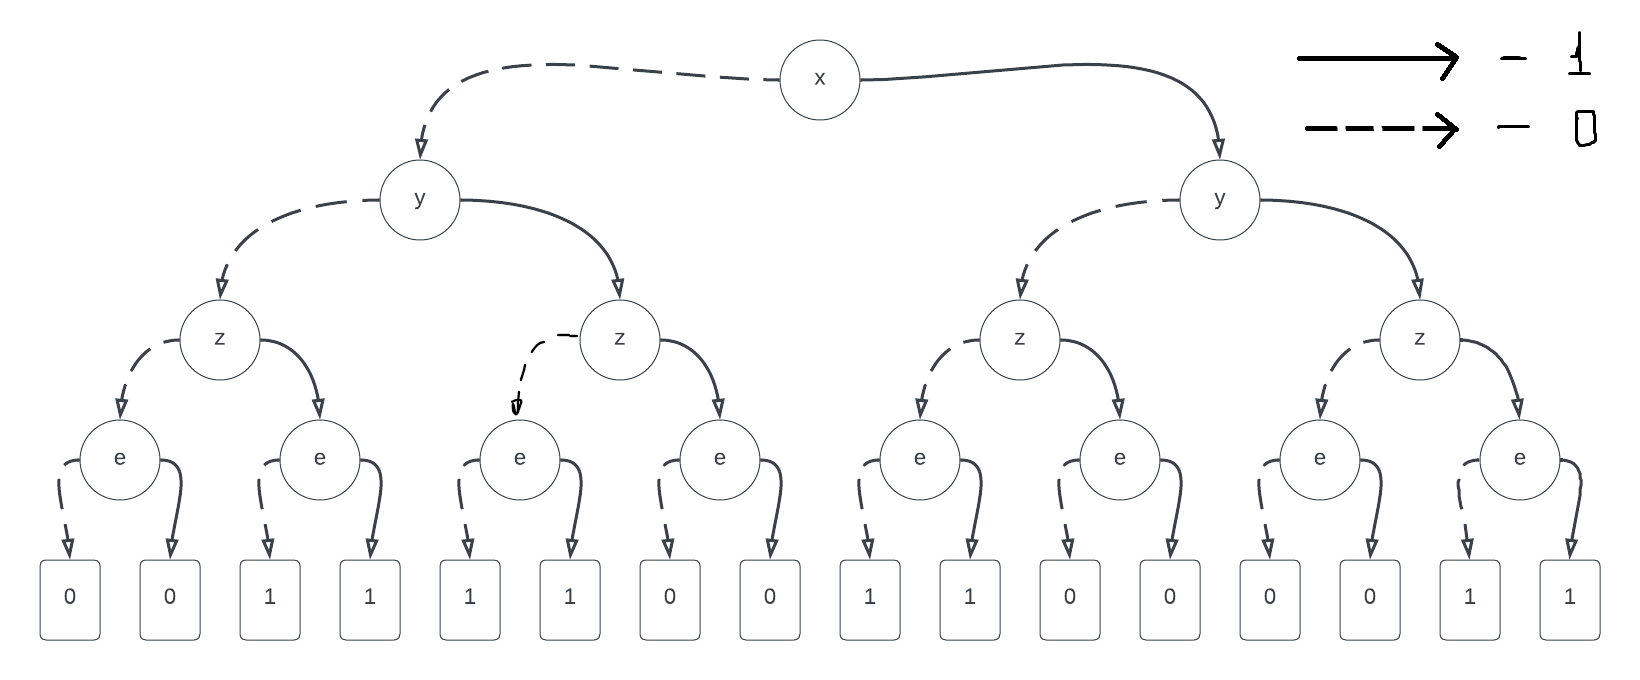
\includegraphics[width=0.8\textwidth]{3}
		\caption{Семантическое дерево.}
	\end{figure}

Семантическое дерево на рисунке 1 можно преобразовать в бинарную диаграмму решений путём применения двух правил сокращения:

\begin{enumerate}[itemsep=0pt,parsep=0pt,topsep=0pt,partopsep=0pt]
	\item Слияние любых изоморфных подграфов.
	\item Удаление всех узлов с изоморфными потомками.
\end{enumerate}

Получившаяся БДР изображена на рисунке 2.

	\begin{figure}[h!]
	\centering
	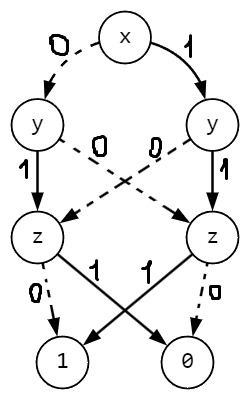
\includegraphics[width=0.2\textwidth]{4}
	\caption{Бинарная диаграмма решений.}
\end{figure}
	
	
\newpage
\subsection{СКНФ}
Совершенная конъюнктивная нормальная форма (СКНФ) - одна из форм представления функции алгебры логики (булевой функции) в виде логического выражения. Представляет собой частный случай КНФ, удовлетворяющий следующим трём условиям:

\begin{enumerate}[itemsep=0pt,parsep=0pt,topsep=0pt,partopsep=0pt]
	\item в ней нет одинаковых множителей (элементарных дизъюнкций);
	
	\item в каждом множителе нет повторяющихся переменных;
	
	\item каждый множитель содержит все переменные, от которых зависит булева функция (каждая переменная может входить в множитель либо в прямой, либо в инверсной форме).
	
\end{enumerate}

Любая булева формула, не являющаяся тождественно истинной, может быть приведена к СКНФ. Также всякая булева функция имеет единственную совершенную конъюктивную нормальную форму (СКНФ). 

$$f(x_1,...,x_n)=\bigwedge_{\{\sigma_1,...,\sigma_n\}|f^*\{\sigma_1,...,\sigma_n\}\}} x_1^{\sigma_1} \land ... \land x_n^{\sigma_n}$$

СКНФ для функции 4-х переменных заданной вектором значений (0011110011000011) будет следующей:	
CKНФf $ =  
(x \lor y \lor z \lor e)\land 
(x \lor y \lor z \lor \overline{e})\land 
(x \lor \overline{y} \lor \overline{z} \lor e)\land 
(x \lor \overline{y} \lor \overline{z} \lor \overline{e})\land 
(\overline{x} \lor y \lor \overline{z}\lor e)\land 
(\overline{x} \lor y \lor \overline{z} \lor \overline{e})\land 
(\overline{x }\lor \overline{y} \lor z \lor e)\land 
(\overline{x} \lor \overline{y} \lor z \lor \overline{e}) $

\subsection{СДНФ}
Совершенная дизъюнктивная нормальная форма (СДНФ) - одна из форм представления функции алгебры логики (булевой функции) в виде логического выражения. Представляет собой частный случай ДНФ, удовлетворяющий следующим трём условиям:

\begin{enumerate}[itemsep=0pt,parsep=0pt,topsep=0pt,partopsep=0pt]
	\item в ней нет одинаковых слагаемых (элементарных конъюнкций);
	
	\item в каждом слагаемом нет повторяющихся переменных;
	
	\item к каждое слагаемое содержит все переменные, от которых зависит булева функция (каждая переменная может входить в слагаемое либо в прямой, либо в инверсной форме).
	
\end{enumerate}

Любая булева формула, не являющаяся тождественно ложной, может быть приведена к СДНФ, причём единственным образом, то есть для любой выполнимой функции алгебры логики существует своя СДНФ, причём единственная.

$$f(x_1,...,x_n)=\bigvee_{\{\sigma_1,...,\sigma_n\}|f\{\sigma_1,...,\sigma_n\}\}} x_1^{\sigma_1} \lor ... \lor x_n^{\sigma_n}$$

СДНФ для функции 4-х переменных заданной вектором значений (0011110011000011) будет следующей:

CДHФf$ = 
\bar{x} y \bar{z} e \lor
\bar{x} y \bar{z} \bar{e} \lor
\bar{x}\bar{y}ze \lor 
\bar{z}\bar{y}z\bar{e} \lor
x\bar{y}\bar{z}\bar{e} \lor
x\bar{y}\bar{z}e \lor
xyz\bar{e} \lor
xyze$

\subsection{Полином Жегалкина}
Полином Жегалкина - многочлен над полем $Z_{2}$, то есть полином с коэффициентами вида 0 и 1 , где в качестве произведения берётся конъюнкция, а в качестве сложения - исключающее или. Полином был предложен в 1927 году Иваном Жегалкиным в качестве удобного средства для представления функций булевой логики.

Ормально полином Жегалкина можно представить в следующем виде:

$$ P(x_1,...,x_n)=\alpha_0a_1 \oplus \alpha_1 x_1 \oplus \alpha_2 x_2 \oplus ... \oplus \alpha_{2^n-1}x_1x_2...x_n$$


Полином Жегалкина для функции 4-х переменных заданной вектором значений (0011110011000011) будет следующим:

$$
\operatorname{Pf}= x \oplus y \oplus z 
$$


\subsection{Дерево решений}
На рисунке 3 изображено дерево решений для функции 4 -х переменных заданной вектором значений (0011110011000011), с порядком переменных xyze.
	\begin{figure}[h!]
	\centering
	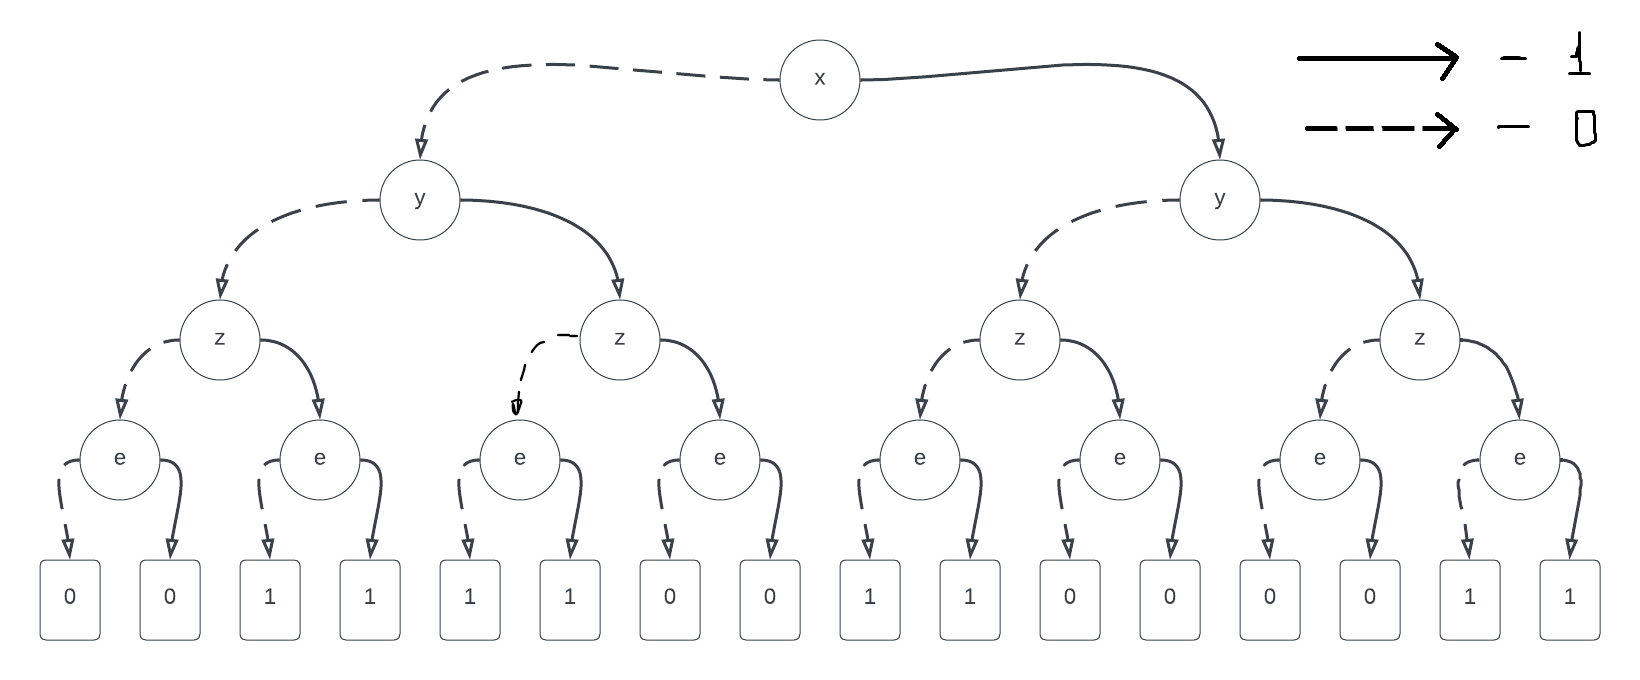
\includegraphics[width=0.8\textwidth]{3}
	\caption{Бинарная диаграмма решений.}
\end{figure}


\subsection{Бинарная диаграмма решений}
На рисунке ~\ref{fig:рис4} изображена бинарная диаграмма решений для функции 4 -х переменных заданной вектором значений (0011110011000011), с порядком переменных xyze.



\subsection{Синтаксическое дерево}
На рисунке ~\ref{fig:рис5} изображено синтаксическое дерево, построенное  по минимизированной формуле $ xyz \lor x \bar {y} \bar {z} \lor \bar {x} y \bar {z} \lor\bar{x} \bar{y}z  $, полученной путём сокращения СДНФ для функции 4 -х переменных заданной вектором значений (0011110011000011).

\begin{figure}[h!]
	\centering
	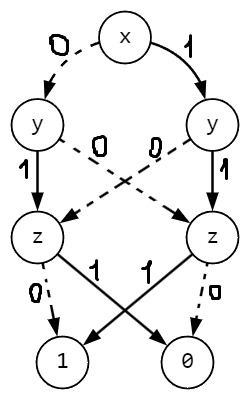
\includegraphics[width=0.2\linewidth]{4}
	\caption{Бинарная диаграмма решений (сплошная линия - для 1 , пунктирная для 0).}
	\label{fig:рис4}
\end{figure}

\begin{figure}[h!]
	\centering
	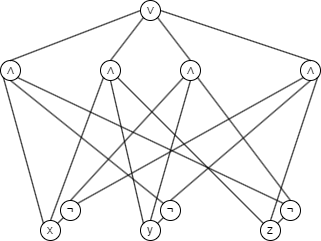
\includegraphics[width=0.8\linewidth]{20}
	\caption{Синтаксическое дерево.}
		\label{fig:рис5}
\end{figure}


\newpage
\section{Особенности реализации}
\subsection{Структура data}
\par Структура создана для помощи хранения Бинарной диаграммы решений в виде бинарного дерева.
 \par Она содержит следующие переменные:
 \begin{enumerate}[itemsep=0pt,parsep=0pt,topsep=0pt,partopsep=0pt]
 	\item char name -- переменная для хранения названия
 	\item data* False -- указатель на структуру: отвлетление -- 0. 
 	\item data* True;  указатель на структуру: отвлетление -- 1. 
 	\end{enumerate}
% 	\subsubsection{Конструктор data и методы AddTrue,AddFalse}
 %	\par Вход:            
 %	\par 
 %	\par В конструкторе переменной с именем name присваивается "s", двум указателям присваивается пустой указатель "nullptr"
 	
% 	\begin{lstlisting}[caption={Конструктор data}]
 %	data(const char s) {
 %		name = s;
 %		False = nullptr;
 %		True = nullptr;
 %	}
 %	\end{lstlisting}
 	
 %	\par Метод AddTrue, присваивает конечной вершине 

\subsection{Класс Tabl} 
\par Класс Tabl -- основной класс в данной лабораторной работе. Он отвечает за хранение и доступ к таблице истинности, СДНФ, СКНФ, БДР и полиному Жегалкина.
\par В классе присутствуют переменные:
\begin{enumerate}[itemsep=0pt,parsep=0pt,topsep=0pt,partopsep=0pt]
	\item vector<bool> x -- массив отвечающий за столбец x в таблице истинности.
	\item vector<bool> y -- массив отвечающий за столбец y в таблице истинности.
	\item vector<bool> z -- массив отвечающий за столбец z в таблице истинности.
	\item vector<bool> e -- массив отвечающий за столбец e в таблице истинности.
	\item vector<bool> f -- массив отвечающий за столбец f в таблице истинности.
	\item data* BDR -- указатель на объект структуры, необходим, для хранения БДР: верхушку бинарного дерева.
	\item string SDNF -- строка содержащая СДНФ.
	\item string SKNF -- строка содержащая СКНФ.
	\item vector <vector<bool>> Zhegalkin -- двумерный массив, хранящий полином жегалкина в виде таблицы.
	\item vector <int> Alpha\_index -- массив хранящий индексы $\alpha_i$ в определенном порядке.  
	\item string Zhegalkin\_str --строка содержащая полином жигалкина в виде выражения.
\end{enumerate}

\subsubsection{Конструктор Tabl}
\par Вход: создание таблицы истинности, СДНФ, СКНФ, БДР и полинома Жегалкина
\par Выход: сформированные таблица истинности, СДНФ, СКНФ, БДР и полином Жегалкина.
\par Вначале составляется таблица истинности с помощью цикла for. В столбец x, то есть в массив x, ставится "0" если i<8, иначе "1". В массив y ставится "1", если i кратна либо 4, либо 5, либо 6, либо 7, иначе "0". В столбец z ставится "1", когда i кратна либо 2, либо 3, в другох случаях "0". В е ставится "1", если i-- нечетное, иначе "0". 

\par Далее создаются вершины дерева БДР, и соединяются друг с другом, с помощью указалей в стрктуре data, в соответсвии с БДР начерченной на листке.

\par После с помощью цикла for заполняются строки СДНФ и СКНФ, опираясь на данные таблицы истинности.

\par Следующим шагом заполняется двумерный массив полинома жигалкина в виде таблицы, тоже с помощью цикла for. Также заполняется массив коэффициэнтов $\alpha_i$ в специальном порядке, которые соответствует формуле: $\operatorname{Pf}=\alpha_0 \oplus\alpha_1x \oplus\alpha_2y \oplus\alpha_3z  \oplus\alpha_4e\oplus\alpha_5xy\oplus\alpha_6xz\oplus\alpha_7xe\oplus\alpha_8yz\oplus\alpha_9ye\oplus\alpha_{10}ze\oplus\alpha_{11}xyz\oplus\alpha_{12}xye\oplus\alpha_{13}xze\oplus\alpha_{14}yze\oplus\alpha_15xyze $. После по данной таблице строится полином жегалкина в виде выражения.
\par Код контруктора ниже, в листинге 1. 

\begin{lstlisting}[caption={Конструктор Tabl}]
	Tabl::Tabl() {
		x.resize(16, 0);
		y.resize(16, 0);
		z.resize(16, 0);
		e.resize(16, 0);
		f.resize(16, 0);
		
		int kx = 0, ky = 0, kz = 0, ke = 0;
		for (int i = 0; i < 16; i++) {
			
			x[i] = i < 8 ? 0 : 1;
			
			y[i] = (i & 4) == 4 || (i & 5) == 5 || (i & 6) == 6 || (i & 7) == 7 ? 1 : 0;
			
			z[i] = (i & 2) == 2 || (i & 3) == 3 ? 1 : 0;
			
			e[i] = i & 1 ? 1 : 0;
			
			f[i] = i == 2 || i == 3 || i == 4 || i == 5 || i == 8 || i == 9 || i == 14 || i == 15 ? 1 : 0;
		}
		
		BDR = new data('x');
		
		data* BDR_y0 = new data('y');
		data* BDR_y1 = new data('y');
		BDR->AddFalse(BDR_y0);
		BDR->AddTrue(BDR_y1);
		
		data* BDR_z0 = new data('z');
		data* BDR_z1 = new data('z');
		
		BDR_y0->AddFalse(BDR_z1);
		BDR_y0->AddTrue(BDR_z0);
		
		BDR_y1->AddFalse(BDR_z0);
		BDR_y1->AddTrue(BDR_z1);
		
		data* BDR_0 = new data('0');
		data* BDR_1 = new data('1');
		
		BDR_z0->AddFalse(BDR_1);
		BDR_z0->AddTrue(BDR_0);
		
		BDR_z1->AddFalse(BDR_0);
		BDR_z1->AddTrue(BDR_1);
		
		SDNF = "СДНФ = ";
		SKNF = "СКНФ = ";
		for (int i = 0, k1=0,k2=0; i < 16; i++) {
			if (f[i] == 1) {
				SDNF += x[i] == 1 ? "x " : "!x ";
				SDNF += y[i] == 1 ? "y " : "!y ";
				SDNF += z[i] == 1 ? "z " : "!z ";
				SDNF += e[i] == 1 ? "e " : "!e ";
				SDNF += k1 < 7 ? " V  " : "\0";
				k1++;
			}
			else {
				SKNF += "(";
				SKNF += x[i] == 0 ? "x" : "!x";
				SKNF += " V ";
				SKNF += y[i] == 0 ? "y" : "!y";
				SKNF += " V ";
				SKNF += z[i] == 0 ? "z" : "!z";
				SKNF += " V ";
				SKNF += e[i] == 0 ? "e" : "!e";
				SKNF += ")";
				SDNF += k2 < 7 ? "" : "\0";
				k2++;
			}
		}
		
		for (int i = 16; i >0; i--) {
			std::vector <bool> buf(i);
			Zhegalkin.push_back(buf);
		}
		for (int i = 0; i < 16; i++) {
			Zhegalkin[0][i] = f[i];
		}
		for (int i = 1; i < 16; i++) {
			for (int j = 0; j < Zhegalkin[i].size(); j++) {
				Zhegalkin[i][j] = Zhegalkin[i - 1][j] == Zhegalkin[i - 1][j + 1] ? 0 : 1;
			}
		}
		
		Alpha_index.push_back(0);
		Alpha_index.push_back(4);
		Alpha_index.push_back(3);
		Alpha_index.push_back(10);
		Alpha_index.push_back(2);
		Alpha_index.push_back(9);
		Alpha_index.push_back(8);
		Alpha_index.push_back(14);
		Alpha_index.push_back(1);
		Alpha_index.push_back(7);
		Alpha_index.push_back(6);
		Alpha_index.push_back(13);
		Alpha_index.push_back(5);
		Alpha_index.push_back(12);
		Alpha_index.push_back(11);
		Alpha_index.push_back(15);
		
		Zhegalkin_str = "F = ";
		for (int i = 0; i < 16; i++) {
			if (Zhegalkin[i][0] == 1) {
				Zhegalkin_str += "a_";
				Zhegalkin_str += std::to_string(Alpha_index[i]);
				Zhegalkin_str += " ";
				Zhegalkin_str += x[i] == 1 ? "x" : "";
				Zhegalkin_str += y[i] == 1 ? "y" : "";
				Zhegalkin_str += z[i] == 1 ? "z" : "";
				Zhegalkin_str += e[i] == 1 ? "e" : "";
				Zhegalkin_str += i < 15 ? " + " : "\0";
			}
		}
	}
\end{lstlisting}
\subsubsection{Метод Print}
\par Вход: намерение отобразить  таблицу истинности на консоль. 
\par Выход: отображение таблицы истинности на консоли.
\par Метод Print выводит на экран таблицу истинности.

\begin{lstlisting}[caption={Метод Print}]
void Tabl::Print() {
	std::cout << "  " << "x y z e \textbar f" << std::endl;
	std::cout << "  -----------\n";

	for (int i = 0; i < 16; i++) {
		std::cout << "  " << x[i] << " " << y[i] << " " << z[i] << " " << e[i] <<" \textbar " << f[i] << std::endl;
	}
}
\end{lstlisting}


\subsubsection{Метод Print\_SKNF}
\par Вход: намерение отобразить  СКНФ и на консоль. 
\par Выход: отображение СКНФ на консоли.
\par Метод Print\_SKNF выводит на экран СКНФ.
\begin{lstlisting}[caption={Метод Print\_SKNF}]
		void Tabl::Print_SKNF() {
			std::cout << std::endl<<SKNF << std::endl;
		}
\end{lstlisting}

\subsubsection{Метод Print\_SDNF}
\par Вход: намерение отобразить  СДНФ и на консоль. 
\par Выход: отображение СДНФ на консоли.
\par Метод Print\_SDNF выводит на экран СДНФ.
\begin{lstlisting}[caption={Метод Print\_SDNF}]
void Tabl::Print_SDNF() {
	std::cout << std::endl<<SDNF << std::endl;
}
\end{lstlisting}

\subsubsection{Метод Print\_Zhegalkin}
\par Вход: намерение отобразить  полином Жегалкина и на консоль. 
\par Выход: отображение полинома Жегалкина на консоли.
\par Метод Print\_Zhegalkin выводит на экран полином Жегалкина, то есть строит таблицу, и ниже пишет сам полином.
\begin{lstlisting}[caption={Метод Print\_Zhegalkin}]
void Tabl::Print_Zhegalkin() {
	std::string s = " ";
	std::printf(" Полином Жегалкина:\n");
	std::printf(" -----------------\n");
	
	for (int i = 0; i < 16; i++) {
		std::cout << "a_" << Alpha_index[i] <<'\t' << s;
		s += " ";
		for (int j = 0; j < Zhegalkin[i].size(); j++) {
			std::cout << Zhegalkin[i][j] << " ";
		}
		std::printf("\n");
	}
	std::cout <<std::endl<< Zhegalkin_str<<std::endl;
}
\end{lstlisting}

\subsubsection{Метод Search\_SDNF}
\par Вход: булева функция, которую вводит пользователь.
\par Выход: вывод на консоль значения булевой функции.
\par В методе Search\_SDNF происходит подставление элементов булевой функции в строчку СДНФ, затем подсчет выражение, и получение результата.
\begin{lstlisting}[caption={Метод Search\_SDNF}]
	void Tabl::Search_SDNF(std::string s) {
		std::string s_out = "";
		
		for (int i = 0; i < 4; i++) {
			s_out += s[i] == '0' ? "1" : "0";
		}
		
		std::string buf="";
		
		for (int i = 0; SDNF[i] != '\0'; i++) {
			buf += SDNF[i] == 'x' ? SDNF[i - 1] == '!' ? std::string(1, s_out[0]) : std::string(1, s[0]) : "";
			buf += SDNF[i] == 'y' ? SDNF[i - 1] == '!' ? std::string(1, s_out[1]) : std::string(1, s[1]) : "";
			buf += SDNF[i] == 'e' ? SDNF[i - 1] == '!' ? std::string(1, s_out[3]) : std::string(1, s[3]) : "";
			buf += SDNF[i] == 'V' ? "+" : "";
			buf += SDNF[i + 1] == '\0' ? "+!\0" : "";
		}
		
		std::vector<int> result;
		
		for (int i = 0, k = 0; buf[i] != '!'; i += 5) {
			result.push_back(1);
			result[k] &= buf[i] == '1' ? 1 : 0;
			result[k] &= buf[i + 1] == '1' ? 1 : 0;
			result[k] &= buf[i + 2] == '1' ? 1 : 0;
			result[k] &= buf[i + 3] == '1' ? 1 : 0;
			k++;
		}
		int Result=0;
		for (int i = 0; i < result.size(); i++) {
			Result \textbar=  result[i];
		}
		std::cout << "\tОтвет: " << Result << std::endl;
	}
	
\end{lstlisting}

\subsubsection{Метод Search\_Zhegalkin};

\par Вход: булева функция, которую вводит пользователь.
\par Выход: вывод на консоль значения булевой функции.
\par В методе  Search\_Zhegalkin происходит подставление элементов булевой функции в строчку полинома Жегалкина, затем подсчет выражение, и получение результата.
\begin{lstlisting}[caption={Метод Search\_Zhegalkin}]
	void Tabl::Search_Zhegalkin(std::string s) {
		std::string buf = "";
	
		for (int i = 0; Zhegalkin_str[i] != '\0'; i++) {
			buf += Zhegalkin_str[i] == 'x' ? std::string(1,s[0]) : "";
			buf += Zhegalkin_str[i] == 'y' ? std::string(1,s[1]) : "";
			buf += Zhegalkin_str[i] == 'z' ? std::string(1,s[2]) : "";
			buf += Zhegalkin_str[i] == 'e' ? std::string(1,s[3]) : "";
			buf += Zhegalkin_str[i] == '+' ? "+" : "";
		}
		
		bool result=buf[0]=='0'?0:1;
		bool buffer= buf[2] == '0' ? 0 : 1;
		bool buffer1= buf[4] == '0' ? 0 : 1;
		result = result != buffer ? 1 : 0;
		result = result != buffer1 ? 1 : 0;
	
		std::cout << "\tОтвет: " << result << std::endl;
	}
\end{lstlisting}


\subsubsection{Метод Search}

\par Вход: булева функция, которую вводит пользователь.
\par Выход: вывод на консоль значения булевой функции.
\par В методе  Search происходит поиск в БДР решения по булевой функции, затем получнение результата, и вывод на консоль.
\begin{lstlisting}[caption={Метод Search}]
void Tabl::Search(std::string s) {
	
	data* buf = this->BDR;
	
	for (int i = 0; i < 3; i++) {
		if (s[i] == '0')
		buf = buf->False;
		if (s[i] == '1')
		buf = buf->True;
	}
	std::printf("\tОтвет: %c\n", buf->name);
}
\end{lstlisting}


\subsubsection{Метод Check}

\par Вход: булева функция, которую вводит пользователь.
\par Выход: вывод булевой функции по таблице истинности.
\par В методе  Check происходит поиск в таблице истинности решения по булевой функции, после происходит вывод данного результата. Это необходимо для автоматической проверки с таблицей истинности в других методах, где происходит поиск результата по БДР, СДНФ и полиному Жегалкина.
\begin{lstlisting}[caption={Метод Check}]
	bool Tabl::Check(std::string s) {
		bool result = 0;
		bool s_0 = s[0] == '0' ? 0 : 1;
		bool s_1 = s[1] == '0' ? 0 : 1;
		bool s_2 = s[2] == '0' ? 0 : 1;
		bool s_3 = s[3] == '0' ? 0 : 1;
		
		for (int i = 0; i < 16; i++)
		if (x[i] == s_0)
		if (y[i] == s_1)
		if (z[i] == s_2)
		if (e[i] == s_3) {
			result = f[i];
			return result;;
		}
	}
\end{lstlisting}

\subsubsection{Метод CheckInput\_Menu}

\par Вход: ожидание правильного ввода пользователя для работы в дальнейшем, а именно выбора действия в меню.
\par Выход: вывод возможный номер действия из меню действий.
\par В методе  CheckInput\_Menu происходит проверка на корректность пользовательского ввода. Данный метод при помощи цикла while заставляет пользователя вводить значение заново, пока оно не будет корректным. Для проверки используется диапазон от 0 до 7 вкючительно и try catch,если пользователь введет вместо цифру любой другой символ. 
\begin{lstlisting}[caption={Метод CheckInput\_Menu}]
	std::string Tabl::CheckInput_Menu() {
		std::string s;
		
		while (true) {
			std::cin >> s;
		
			try {
				if (stoi(s) >= 0 && stoi(s) <= 7) {
					break;
				}
				else {
					std::cout << "Ошибка ввода! Ведите число от 0 до 7\n";
				}
			}
			catch (const std::invalid_argument& e) {
				std::cout << "Ошибка ввода! Неверный формат числа\n";
			}
		}
		return s;
	}
\end{lstlisting}


\subsubsection{Метод CheckInput}

\par Вход: ожидание правильного ввода пользователя для работы в дальнейшем, а именно булевой функции.
\par Выход: булевая функция пригодная для использования.
\par В методе  CheckInput происходит проверка на корректность пользовательского ввода. Данный метод при помощи цикла while заставляет пользователя вводить значение заново, пока оно не будет корректным. Для проверки используется регулярное выражение в котором необходимо вводить либо 0, либо 1, и всего цифр должно быть 4, иначе  пользователю необходимо вводить булеву функции заново.
\begin{lstlisting}[caption={Метод CheckInput}]
	std::string Tabl::CheckInput() {
		std::regex BDR("^[0-1]{4}$");
		std::string s;
		std::printf("\nВведите значения переменных x, у, z, e в однустрочку без пробелов (пример: 1010)\n");
		while (true) {
			std::cin >> s;
			if (regex_match(s, BDR))
				break;
			else
				std::printf("Ошибка в вводе, попробуйте снова\n");
		}
		return s;
	}
\end{lstlisting}

\subsubsection{Menu}

\par Вход: ожидание вывести возможные действия работы программы пользователю.
\par Выход: выводится меню действий на консоль, позьзователь выбирает нужное для него действие.
\par В методе  Menu происходит вывод на экран всех возможных действий. Пользователь выбирает  нужное ему действие, при этом вызывается метод для проверки пользовательсктго ввода, дальше вызывается метот соответствующий выбору пользователя.
\begin{lstlisting}[caption={Метод Menu}]
	void Tabl::Menu() {
		while (true) {
			printf("\nВыберите что вы хотите:\n");
			printf(" [1]\tВывести на экран таблицу истинности\n");
			printf(" [2]\tПолином Жегалкина\n");
			printf(" [3]\tСДНФ\n");
			printf(" [4]\tСКНФ\n");
			printf(" [5]\tНайти значение по БДР\n");
			printf(" [6]\tНайти значение по СДНФ\n");
			printf(" [7]\tНайти значение по полиному Жегалкина\n");
			printf(" [0]\tВыход\n");
			
			std::string s;
			
			s = CheckInput_Menu();
			
			bool Out = 0;
			
			switch (stoi(s)) {
				case 0:
					Out = 1;
					break;
					
				case 1:
					Print();
					break;
					
				case 2:
					Print_Zhegalkin();
					break;
			
				case 3:
					Print_SDNF();
					break;
			
				case 4:
					Print_SKNF();
					break;
			
				case 5:
					s = CheckInput();
					Search(s);
					break;
			
				case 6:
					s = CheckInput();
					Search_SDNF(s);
					break;
			
				case 7:
					s = CheckInput();
					Search_Zhegalkin(s);
					break;
			}
			if (Out)
				break;
			system("pause");
		}
	}
\end{lstlisting}

\newpage
\section{Результаты работы программы}

При запуске программы на консоль выводится главное меню с перечнем возможных действий, которые может выбрать пользователь (рисунок 6).
	\begin{figure}[h!]
	\centering
	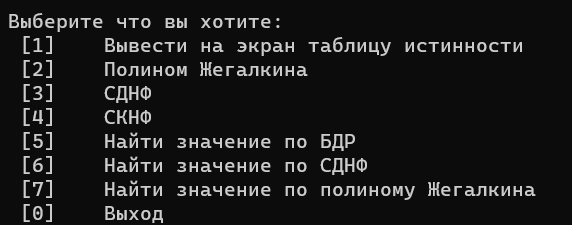
\includegraphics[width=0.8\textwidth]{7}
	\caption{Главное меню программы}
\end{figure}

После нажатия клавиши <<1>>, либо <<2>>, либо <<3>>, либо <<4>>, на консоль выводится таблица истинности, полином Жегалкина, СДНФ, СКНФ соответственно  (рисунки 7-10).
	\begin{figure}[h!]
			\centering
	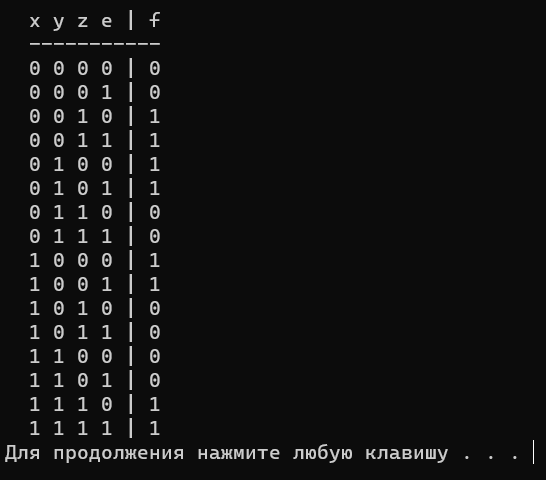
\includegraphics[width=0.8\textwidth]{6}
	\caption{Таблица истинности.}
\end{figure}
	\begin{figure}[h!]
			\centering
	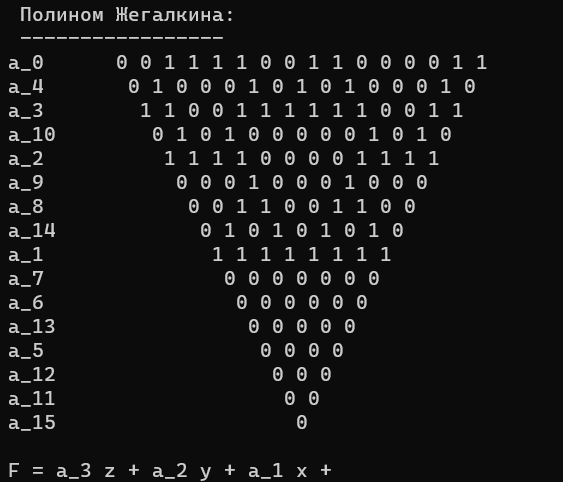
\includegraphics[width=0.8\textwidth]{8}
	\caption{Полином Жегалкина.}
	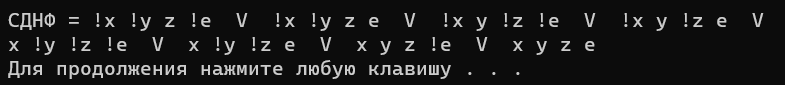
\includegraphics[width=0.8\textwidth]{9}
	\caption{СДНФ}
	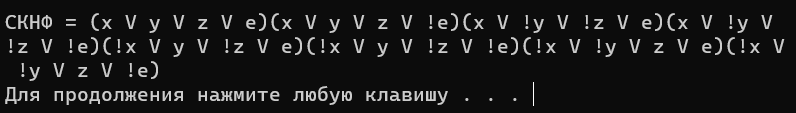
\includegraphics[width=0.8\textwidth]{10}
	\caption{СКНФ}
\end{figure}	
\clearpage

При нажатии клавиши  <<5>>, либо <<6>>, либо <<7>>, у пользователя запрашивается булева функция, после происходит вывод результата который производился поиском по БДР, СДНФ и полиному Жегалкина соответственно, а также автоматическая проверка значения по таблице истинности (рисунки 11-13).
	\begin{figure}[h!]
	\centering
	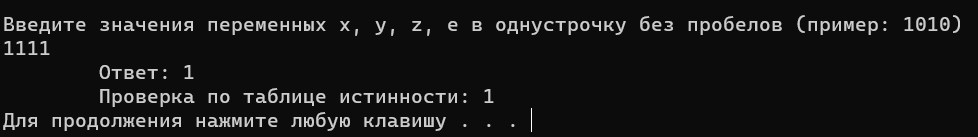
\includegraphics[width=0.8\textwidth]{11}
	\caption{Вывод значения булевой функции 1111 по БДР с проверкой по таблице истинности.}
	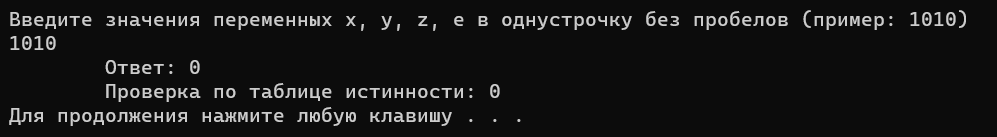
\includegraphics[width=0.8\textwidth]{12}
	\caption{Вывод значения булевой функции 1010 по СДНФ с проверкой по таблице истинности.}
	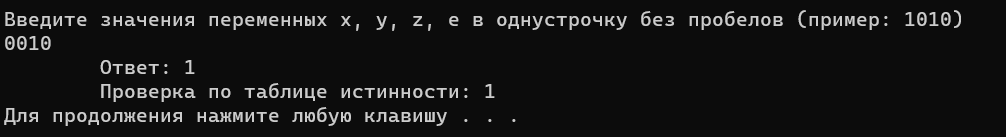
\includegraphics[width=0.8\textwidth]{13}
	\caption{Вывод значения булевой функции 0010 по полиному Жегалкина с проверкой по таблице истинности.}
\end{figure}	

На рисунках 14-15 изображены возможные ошибки при некорректном пользовательском вводе.
	\begin{figure}[h!]
	\centering
	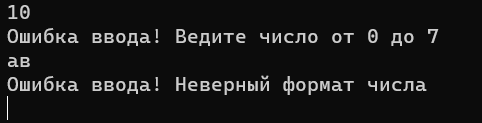
\includegraphics[width=0.6\textwidth]{14}
	\caption{Ввод номера действия, которого нет в меню и ввод не цифры, а любого другого символа.}
	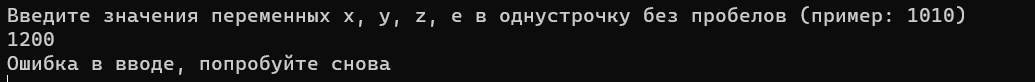
\includegraphics[width=0.8\textwidth]{15}
	\caption{Ввод некоректного булевой функции.}
\end{figure}	
\clearpage
\section* {Заключение}
\addcontentsline{toc}{section}{Заключение}

В ходе выполнения лабораторной работы №2 была реализована программа, вычисляющая по заданному вектору-столбцу значений функции 4-х переменных СДНФ, СКНФ и полином Жегалкина. Программа также  хранит бинарную диаграмму решений, вычисляет по СДНФ, БДР и полиному Жегалкина значение функции и сверяет его с таблицей истинности. В программе реализована защита от некорректного пользовательского ввода. Также отчёте
представлены, построенные вручную, дерево решений, бинарная диаграмма решений и синтаксическое дерево.

Достоинством реализованной программы является объектно-ориентированный подход. Класс Tabl и структура data независимы от внешних параметров, их можно использовать в других программах и совмещать с другими классами.

Из недостатков, я считаю то, что эта реализация расчитана на функцию четырех переменных, при изменении количества переменных, придется достаточно много изменить в коде уже реализованной программы. можно считать, что это узконаправленная реализация. Также недостатком является то, что при вводе тождественно истинной или тождественно ложной функции, программа не будет генерировать строковое представление СКНФ. В случае ввода тождественно ложной функции не будет генерироваться строковое представление СДНФ.

Данную реализацию возможно расширять, без изменении основного функционала существующего кода. Например, можно реализовать построении СДНФ,СКНФ, полинома Жегалкина по введеному пользователем вектору-столбцу значений функции. Также возможно построения базиса Шеффера или базиса Пирса.Все это показывает о способности к расширении данной программы. 

Лабораторная работа реализована на языке С++, в среде разработки Visual Studio 2022.

\newpage
\section* {Источники}
\addcontentsline{toc}{section}{Источники}
\begin{quote}
	1. Дискретная математика для программистов. 3-е издание. Новиков Ф.А.
	СПБ:.Питер,2009.
\end{quote}
	\end{document}